\chapter{Volume Average Method}
\label{ch:vans}

\chapquote{Do not worry about your difficulties in mathematics; I can assure you that mine are still greater.}{Letter to junior high school student Barbara Wilson, \\ January 7, 1943}{Albert Einstein}

\section{Introduction}

Maximum 10 lines recalling some of the things said in the previous chapter.

\section{Derivation of VANS equations for 3D incompressible fluids}
%The dynamic of the liquid phase indicated with the subscript $\beta$ is governed by the Navier-Stokes equation for incompressible Newtonian fluid, in presence of a porous medium solid; the equation valid inside the liquid phase are:
%
%\begin{equation}
%\dfrac{\partial \vb}{\partial t} + \vb \cdot \nabla \vb = -\frac{1}{\rho_{\beta}} \nabla \pb + \nub \nabla^2  \vb  + \mathbf{f}, 
%\label{eq:mom}
%\end{equation}
%\begin{equation}
%\nabla \cdot \vb = 0,
%\label{eq:cont}
%\end{equation}
%where $\vb$, $\pb$, $\rho_{\beta}$ and $\nub$ stand, respectively, for  the velocity, the pressure, the density and the kinematic viscosity of the fluid.

\subsection{Definition of the averaging filter}

In the figure \ref{fig:rev} is an illustration of our porous problem; in the same figure we show all the main definition that we need to introduce in order to develop our mathematical approach.


\begin{figure}[h]
	\centering
	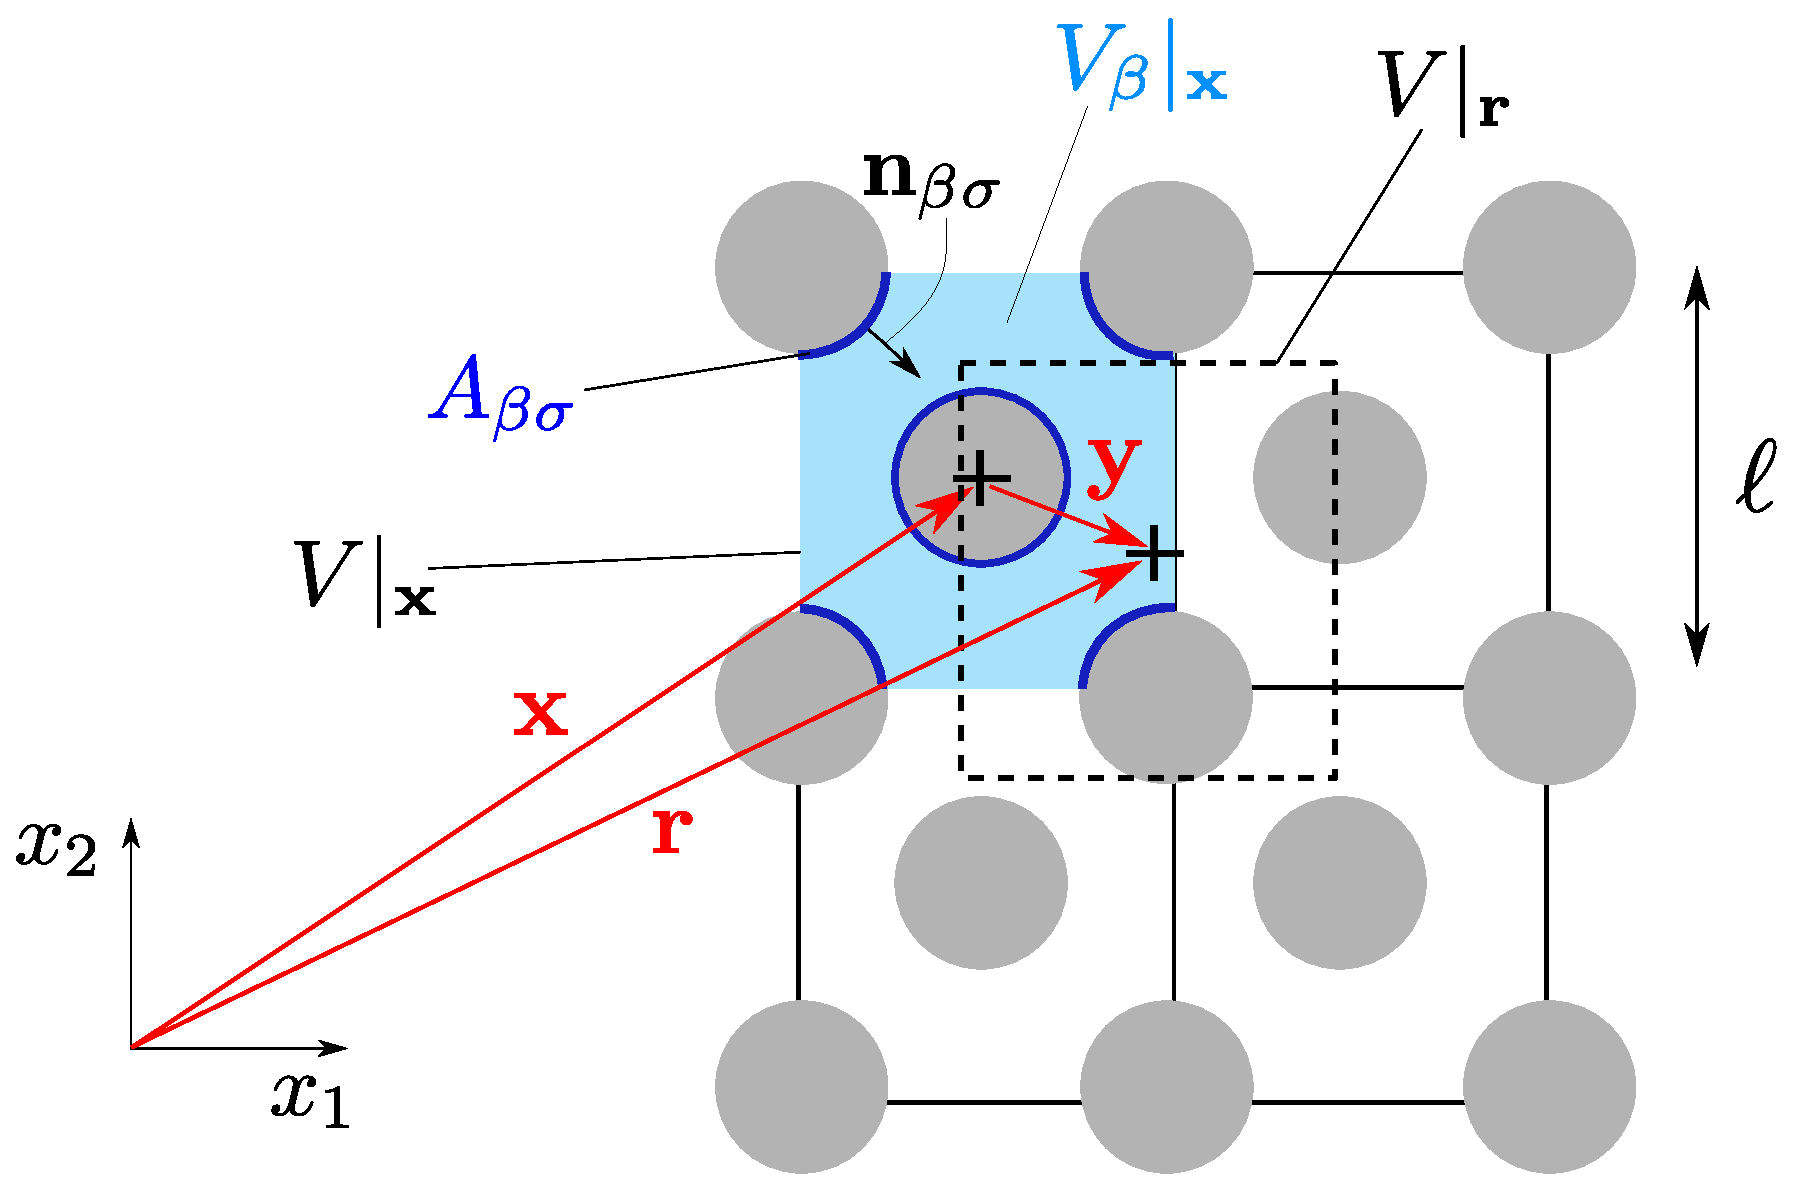
\includegraphics[width=0.7\linewidth]{chapter_2/figure/REV}
	\caption{Illustration of the REV concept.}
	\label{fig:rev}
\end{figure}

Let $\psi_{\beta}$ be an arbitrary vector or scalar field defined on the volume $V$ where $x$ is its centroid, we can define two different spacing average operator.

\begin{equation}
\meani{\psi_{\beta}}|_{\mathbf{x}} = \dfrac{1}{\volb} \int_{\volb(\mathbf{x})}  m(\mathbf{y}) \psi_{\beta}(\mathbf{x}-\mathbf{y}, t) d \, \volb,
\label{eq:avg_intrinsic}
\end{equation}

\begin{equation}
\means{\psi_{\beta}}|_{\mathbf{x}} = \dfrac{1}{V} \int_{\volb} m(\mathbf{y}) \psi_{\beta}(\mathbf{x}-\mathbf{y}, t) d \, \volb,
\label{eq:avg_superficial}
\end{equation}

$\meani{\psi_{\beta}}$ is called the \textit{intrinsic average} and $\means{\psi_{\beta}}$ is the \textit{superficial average}.
For the sake of a less heavy notation the $|_{\mathbf{x}}$ has been dropped in the following, within mind that the volume averaged quantities are intended to be computed in the center of the REV.
The filter $m$ act as a ... it is required that
$$
\int_{\volb(\mathbf{x})}  m(\mathbf{y}) d \, \volb = 1
$$

Also for the sake of simplicity we will consider a filter $m$ to be rectangular and wi will not maintain it in the formulation...

The porosity is defined as:
\begin{equation}
	\varepsilon = \dfrac{\volb}{V}
	\label{eq:porosity}
\end{equation}

So we can defy the relationship:
\begin{equation}
	\means{\psi_{\beta}} =  \varepsilon \meani{\psi_{\beta}}
\end{equation}

\subsection{Theorems involving derivatives of spatial averaging}

\begin{theorem}[Spatial averaging theorem]
Let $\psi_{\beta}$ be a scalar quantity defined in the liquid phase $\beta$, then:
	\begin{equation}
		\means{\nabla \psi_{\beta}} = \nabla \means{\psi_{\beta}} + \dfrac{1}{V} \int_{A_{\beta \sigma}} \psi_{\beta} \mathbf{n}_{\beta \sigma}  dA
			\label{th:spat_avg}
	\end{equation}
\end{theorem}

\begin{corollary}[Vector form of \ref{th:spat_avg}]
	The vector form of the spatial averaging theorem is given by:
	\begin{equation}
	\means{\nabla \cdot \boldsymbol{\psi_{\beta}}} = \nabla \cdot \means{  \boldsymbol{\psi_{\beta}}} + \dfrac{1}{V} \int_{A_{\beta \sigma}} \boldsymbol{n_{\beta \sigma}} \cdot \boldsymbol{\psi_{\beta}} dA
			\label{th:vec_spat_avg}
	\end{equation}
\end{corollary}

\begin{corollary}
	Applying the theorem \ref{th:spat_avg} to a constant field $\psi_{\beta} = 1$ we obtain:
	\begin{equation}
		\nabla \varepsilon = - \int_{A_{\sigma \beta}} \mathbf{n_{\sigma \beta}} d \, A,
	\end{equation}
\end{corollary}


\begin{theorem}[General transport theorem]
	Let $\psi_{\beta}$ be a scalar quantity defined in the liquid phase $\beta$, then:
	\begin{equation}
	\dfrac{\partial}{\partial t} \int_{\volb(t)} \psi_{\beta} dV =  \int_{\volb(t)} \dfrac{\partial \psi_{\beta}}{\partial t} dV + \int_{A_{\beta \sigma}(t)} \psi_{\beta} (\mathbf{n}_{\beta \sigma} \cdot \mathbf{w} ) dA,
	\label{th:transport}
	\end{equation}
	
	where $\mathbf{w}$ is the point velocity of the solid-liquid interface $A_{\beta \sigma}$.
\end{theorem}


\subsection{Averaged continuity equations}

The continuity equation for a Newtonian ... reads:

\begin{equation}
\means{\dfrac{\partial \rho_{\beta}}{\partial t}} + \means{\nabla \cdot (\rho_{\beta}\vb)}   = 0
\label{eq:superf_avg_cont}
\end{equation}

Applying \ref{th:spat_avg} to the second term we get:
\begin{equation}
 \means{\nabla \cdot (\rho_{\beta}\vb)} = \nabla \cdot \means{ (\rho_{\beta}\vb)} + \dfrac{1}{V} \int_{A_{\beta \sigma}} \boldsymbol{n_{\beta \sigma}} \cdot \boldsymbol{\rho_{\beta} \vb} dA
 \label{eq:avg_1}
\end{equation}

and applying fist the definition of superficial average, than \ref{th:transport} to the first one:

\begin{eqnarray}
&&\means{\dfrac{\partial \rho_{\beta}}{\partial t}} = \dfrac{1}{V} \int_{V} \dfrac{\partial \rho_{\beta}}{\partial t} dV = \\
&& = \dfrac{1}{V} \left[  \dfrac{\partial}{\partial t} \int_{V} \rho_{\beta} dV -  \int_{A_{\beta \sigma}} \rho_{\beta} (\mathbf{n}_{\beta \sigma} \cdot \mathbf{w} ) dA   \right] \\
&& = \dfrac{\partial \means{\rho_{\beta}}}{\partial t} -\dfrac{1}{V}  \int_{A_{\beta \sigma}} \rho_{\beta} (\mathbf{n}_{\beta \sigma} \cdot \mathbf{w} ) dA 
\label{eq:avg_2}
\end{eqnarray}

The boundary condition at the interface $\mathbf{w} = \vb$ imply that the integrals in \ref{eq:avg_1} is equal to the integral in \ref{eq:avg_2} so we end up with:

\begin{equation}
\derp{\means{\rho_{\beta}}}{t} + \nabla \cdot \means{\rho_{\beta}\vb} = 0
\end{equation}

Adding the hypothesis of incompressible fluid:
\begin{equation}
\derp{\varepsilon}{t} + \nabla \cdot \means{\vb} = 0
\end{equation}



\subsection{Averaged momentum equations}


\begin{equation}
\dfrac{\partial \vb}{\partial t} + \nabla \cdot (\vb\vb) = -\frac{1}{\rho_{\beta}} \nabla \pb + \nub \nabla^2  \vb
\label{eq:mom}
\end{equation}

\subsubsection{first term}

Using theorem \ref{th:transport}:
\begin{equation}
\means{\derp{\vb}{t}} = \derp{\means{\vb}}{t} -\dfrac{1}{V} \int_{A_{\beta \sigma}(t)} (\mathbf{n}_{\sigma \beta} \cdot w) \vb dA,
\end{equation}

\subsubsection{second term}

Using theorem \ref{th:vec_spat_avg}:
\begin{equation}
\means{\nabla \cdot (\vb\vb)} = \nabla \cdot \means{\vb \vb} + \dfrac{1}{V} \int_{A_{\beta \sigma}} \mathbf{n}_{\sigma \beta} \cdot (\vb \vb) dA,
\end{equation}


The boundary condition at the interface $\mathbf{w} = \vb$ imply that the integrals in the last two equations are equals so we end up with the total left end side of the momentum equation:
$$
\derp{\means{\vb}}{t} + \nabla \cdot \means{\vb \vb}
$$

\subsubsection{third term}

Using theorem \ref{th:spat_avg}:

\begin{equation}
\means{-\dfrac{1}{\rho_{\beta}} \nabla \pb } = -\dfrac{1}{\rho_{\beta}} \nabla \means{\pb} -\dfrac{1}{V} \int_{A_{\beta \sigma}} \dfrac{\pb}{\rho_{\beta}} \mathbf{n}_{\sigma \beta} dA,
\end{equation}

\subsubsection{fourth term}
Expressing the $\nabla^2$ operator with the identity $\nabla^2 = \nabla \cdot (\nabla)$ (laplacian = div ( grad)), and applying the theorem \ref{th:vec_spat_avg}:


\begin{equation}
\means{\nub\nabla^2 \vb} = \means{\nub\nabla \cdot \nabla \vb} = \nabla \cdot \means{\nub\nabla \vb} +\dfrac{1}{V} \int_{A_{\beta \sigma}} \mathbf{n}_{\sigma \beta} \cdot \nub \nabla \vb dA,
	\label{eq:4_1}
\end{equation}

Now re-using the theorem \ref{th:vec_spat_avg} on the term $\means{\nabla \vb}$ we get:

\begin{eqnarray}
	&&\eqref{eq:4_1} = \nabla \cdot \nub \nabla \means{\vb} + \nabla \cdot \left( \dfrac{1}{V} \int_{A_{\beta \sigma}} \mathbf{n}_{\sigma \beta} \cdot \nub \vb dA \right) + \dfrac{1}{V} \int_{A_{\beta \sigma}} \mathbf{n}_{\sigma \beta} \cdot \nub \nabla \vb dA = \nonumber \\
	&& = \nub\nabla^2 \means{\vb} +  \nabla \cdot \left( \dfrac{1}{V} \int_{A_{\beta \sigma}} \mathbf{n}_{\sigma \beta} \cdot \nub \vb dA \right) + \dfrac{1}{V} \int_{A_{\beta \sigma}} \mathbf{n}_{\sigma \beta} \cdot \nub \nabla \vb dA
\end{eqnarray}

Before continue the development lets put all the pieces together:

\begin{eqnarray}
&& \derp{\means{\vb}}{t} + \nabla \cdot \means{\vb \vb} = -\dfrac{1}{\rho_{\beta}} \nabla \means{\pb} + \nub\nabla^2 \means{\vb} + \nonumber \\
&& +\dfrac{1}{V} \int_{A_{\beta \sigma}} \left( -\dfrac{\pb}{\rho_{\beta}} \mathbf{n}_{\sigma \beta} + \nub \nabla \vb \cdot \mathbf{n}_{\sigma \beta} \right) dA  +  \nabla \cdot \left( \dfrac{1}{V} \int_{A_{\beta \sigma}} \mathbf{n}_{\sigma \beta} \cdot \nub \vb dA \right)
	\label{eq:vans_2}
\end{eqnarray}


\subsection{Length scale decomposition}

To further simplify the equations we use the decomposition proposed by \citet{gray1975derivation}:
\begin{equation}
\psi_{\beta} = \meani{\psi_{\beta}} + \tilde{\psi}_{\beta}
\end{equation}

The non-homogeneous terms in equation \ref{eq:vans_2}:

\begin{equation}
\means{\vb\vb} = \means{\means{\vb}\means{\vb}} +2\means{\means{\vb}\tilde{\vb}} +\means{\tilde{\vb} \tilde{\vb}}
\label{eq:dec_1}
\end{equation}

Applying the superficial average to the perturbation term is possible to demonstrate that it has null mean:
$$
\means{\tilde{\psi}_{\beta}} = \means{\psi_{\beta}} - \means{\meani{\psi_{\beta}}} = \means{\psi_{\beta}} -\varepsilon \meani{\psi_{\beta}} = 0
$$

Using this results to equation \eqref{eq:dec_1}:

\begin{equation}
\means{\vb\vb} = \varepsilon \meani{\vb}\meani{\vb} +\means{\tilde{\vb} \tilde{\vb}}
\end{equation}

Now expressing the time derivative in the intrinsic form:
$$
\derp{\means{\vb}}{t} = \derp{(\varepsilon\meani{\vb})}{t} = \derp{\varepsilon}{t}\meani{\vb} + \varepsilon \derp{\meani{\vb}}{t}
$$

For each integral term of \ref{eq:vans_2} we first apply the decomposition:

\begin{eqnarray}
\dfrac{1}{V} \int_{A_{\beta \sigma}}  -\dfrac{\pb}{\rho_{\beta}} \mathbf{n}_{\sigma \beta} dA &=& \dfrac{1}{V} \int_{A_{\beta \sigma}}  -\dfrac{1}{\rho_{\beta}} \left(\meani{\pb}  + \tilde{\pb}\right) \mathbf{n}_{\sigma \beta} dA = \nonumber \\
&=& -\dfrac{1}{\rho_{\beta}}\nabla\varepsilon \meani{\pb} - \dfrac{1}{V} \int_{A_{\beta \sigma}} \dfrac{\tilde{\pb}}{\rho_{\beta}} \mathbf{n}_{\sigma \beta} dA
\end{eqnarray}

The same for the other two terms:
\begin{eqnarray}
\dfrac{1}{V} \int_{A_{\beta \sigma}} \nub \nabla \vb \cdot \mathbf{n}_{\sigma \beta} dA &=& \dfrac{1}{V} \int_{A_{\beta \sigma}} \nub \nabla (\meani{\vb} +\tilde{\vb}) \cdot \mathbf{n}_{\sigma \beta} dA =  \nonumber \\
&=& - \nub \nabla \varepsilon \nabla \meani{\vb} + \dfrac{1}{V} \int_{A_{\beta \sigma}} \nub \nabla \tilde{\vb} \cdot \mathbf{n}_{\sigma \beta} dA
\end{eqnarray}

\begin{eqnarray}
&&\nabla \cdot \left( \dfrac{1}{V} \int_{A_{\beta \sigma}} \mathbf{n}_{\sigma \beta} \cdot \nub \vb dA \right) = \nabla \cdot \left( \dfrac{1}{V} \int_{A_{\beta \sigma}} \mathbf{n}_{\sigma \beta} \cdot \nub (\meani{\vb} +\tilde{\vb}) dA \right) =  \nonumber \\
&=& -\nabla \cdot \left( \nub \meani{\vb} \nabla \varepsilon \right) + \dfrac{1}{V} \nabla \cdot \left(\int_{A_{\beta \sigma}}  \nub \mathbf{n}_{\sigma \beta} \tilde{\vb} dA \right) =  \nonumber \\
&=& -\nub  \nabla  \meani{\vb} \nabla \varepsilon -\nub \meani{\vb} \nabla^2 \varepsilon + \dfrac{1}{V} \nabla \cdot \left(\int_{A_{\beta \sigma}}  \nub \mathbf{n}_{\sigma \beta} \tilde{\vb} dA \right)
\end{eqnarray}

Now we need to further develop the remaining terms:



The crucial difference between the superficial and the intrinsic quantities can be found in the averaged version of the continuity equations; in case of porosity that vary spatially only the superficial velocity field is solenoidal.


\section{Closure problems}

\section{Interface condition}

Penalization method \citet{angot1999penalization} used in\cite{bruneau2004passive} \cite{bruneau2008numerical} \cite{bruneau2010coupling}...


We think that using a boundary condition at the interface is not a superior approach nor physically neither mathematically.
Using penalization method the slip velocity at the interface can be computed as well as using a boundary condition, and either methods require a parameter to close the formulation, with the advantage using penalization method that the parameter is the spatial distribution of the porosity field that is trivial to compute known the geometry of the medium.

Also in case of very low Reynolds number the boundary condition can be a necessity since the Stokes equations, for the free fluid, and the Darcy one for the porous media are not mathematically compatible; but for $Re>10$ when the Brinkmann model for the porous media is applicable the two set of equations are of the same order and the continuity of pressure and velocity can be imposed directly.

Also there is evidence in literature through numerical and computational experiments \citet{ochoa2017fluid} that exist a transition zone with the size of the pore scale in which the velocity and pressure have a continuous variation.
